\documentclass[journal]{vgtc}                % final (journal style)
%\documentclass[review,journal]{vgtc}         % review (journal style)
%\documentclass[widereview]{vgtc}             % wide-spaced review
%\documentclass[preprint,journal]{vgtc}       % preprint (journal style)
%\documentclass[electronic,journal]{vgtc}     % electronic version, journal

%% Uncomment one of the lines above depending on where your paper is
%% in the conference process. ``review'' and ``widereview'' are for review
%% submission, ``preprint'' is for pre-publication, and the final version
%% doesn't use a specific qualifier. Further, ``electronic'' includes
%% hyperreferences for more convenient online viewing.

%% Please use one of the ``review'' options in combination with the
%% assigned online id (see below) ONLY if your paper uses a double blind
%% review process. Some conferences, like IEEE Vis and InfoVis, have NOT
%% in the past.

%% Please note that the use of figures other than the optional teaser is not permitted on the first page
%% of the journal version.  Figures should begin on the second page and be
%% in CMYK or Grey scale format, otherwise, colour shifting may occur
%% during the printing process.  Papers submitted with figures other than the optional teaser on the
%% first page will be refused.

%% These three lines bring in essential packages: ``mathptmx'' for Type 1
%% typefaces, ``graphicx'' for inclusion of EPS figures. and ``times''
%% for proper handling of the times font family.

\usepackage{mathptmx}
\usepackage{graphicx}
\usepackage{times}
\usepackage[mathscr]{euscript}
\usepackage{tabularx}
\usepackage[final]{review}
\usepackage{enumitem}
\usepackage{wasysym}
\usepackage{array}
\usepackage{tcolorbox}
\usepackage[switch]{lineno}
\usepackage{nameref}
%\linenumbers
%% We encourage the use of mathptmx for consistent usage of times font
%% throughout the proceedings. However, if you encounter conflicts
%% with other math-related packages, you may want to disable it.

%% This turns references into clickable hyperlinks.
\usepackage[bookmarks,backref=false,linkcolor=blue]{hyperref} %,colorlinks
\hypersetup{
  pdfauthor = {},
  pdftitle = {},
  pdfsubject = {},
  pdfkeywords = {},
  colorlinks=true,
  linkcolor= black,
  citecolor= black,
  pageanchor=true,
  urlcolor = black,
  plainpages = false,
  linktocpage
}

%% If you are submitting a paper to a conference for review with a double
%% blind reviewing process, please replace the value ``0'' below with your
%% OnlineID. Otherwise, you may safely leave it at ``0''.
\onlineid{0}

%% declare the category of your paper, only shown in review mode
\vgtccategory{Research}

%% allow for this line if you want the electronic option to work properly
%\vgtcinsertpkg

%% In preprint mode you may define your own headline.
%\preprinttext{To appear in an IEEE VGTC sponsored conference.}

%% Paper title.

\title{A Framework for Creative Visualization-Opportunities Workshops}

%% This is how authors are specified in the journal style

%% indicate IEEE Member or Student Member in form indicated below
\author{
Ethan Kerzner,
Sarah Goodwin,
Jason Dykes,
Sara Jones,
Miriah Meyer
}
\authorfooter{
%% insert punctuation at end of each item
\item
 Ethan Kerzner and Miriah Meyer are with the University of Utah. \\ E-mail: kerzner@sci.utah.edu and miriah@cs.utah.edu.
\item
 Sarah Goodwin is with the Royal Melbourne Institute of Technology and Monash University. E-mail: sarah.goodwin@monash.edu.
\item
 Jason Dykes and Sara Jones are with City, University of London. \\ E-mail: [j.dykes,s.v.jones]@city.ac.uk.
}

%other entries to be set up for journal
\shortauthortitle{Kerzner \MakeLowercase{\textit{et al.}}: A Framework for Creativity Workshops in Applied Visualization Research}
%\shortauthortitle{Firstauthor \MakeLowercase{\textit{et al.}}: Paper Title}

\abstract{Applied visualization researchers often work closely with domain collaborators to explore new and useful applications of visualization. The early stages of collaborations are typically time consuming for all stakeholders as researchers piece together an understanding of domain challenges from disparate discussions and meetings. A number of recent projects, however, report on the use of creative visualization-opportunities (CVO) workshops to accelerate the early stages of applied work, eliciting a wealth of requirements in a few days of focused work. Yet, there is no established guidance for how to use such workshops effectively. In this paper, we present the results of a 2-year collaboration in which we analyzed the use of 17 workshops in 10 visualization contexts. Its primary contribution is a framework for CVO workshops that: 1) identifies a process model for using workshops; 2) describes a structure of what happens within effective workshops; 3) recommends \numberOfGuidelines actionable guidelines for future workshops; and 4) presents an example workshop and workshop methods. The creation of this framework exemplifies the use of critical reflection to learn about visualization in practice from diverse studies and experience.}

%% Keywords that describe your work. Will show as 'Index Terms' in journal
%% please capitalize first letter and insert punctuation after last keyword
\keywords{User-centered visualization design, design studies, creativity workshops, critically reflective practice.}

%% ACM Computing Classification System (CCS). 
%% See <http://www.acm.org/class/1998/> for details.
%% The ``\CCScat'' command takes four arguments.

\CCScatlist{ % not used in journal version
 \CCScat{K.6.1}{Management of Computing and Information Systems}%
{Project and People Management}{Life Cycle};
 \CCScat{K.7.m}{The Computing Profession}{Miscellaneous}{Ethics}
}

%% Uncomment below to include a teaser figure.
%\teaser{
%\centering
%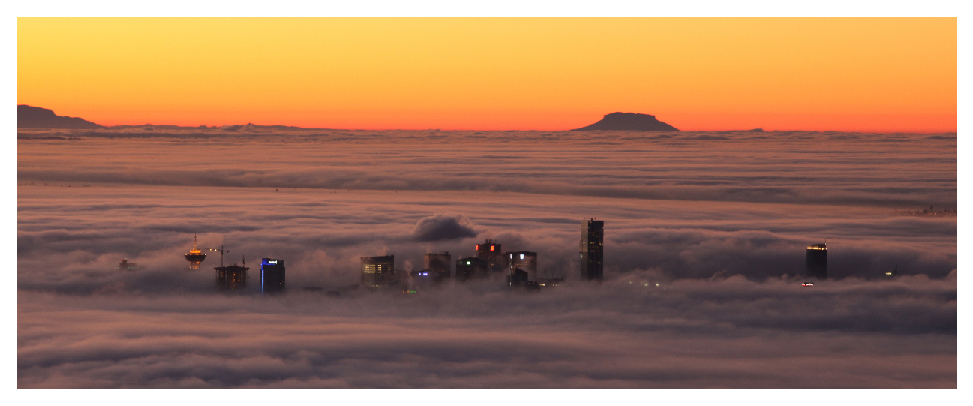
\includegraphics[width=16cm]{CypressView}
%\caption{In the Clouds: Vancouver from Cypress Mountain.}
%}

%% Uncomment below to disable the manuscript note
%\renewcommand{\manuscriptnotetxt}{}

%% Copyright space is enabled by default as required by guidelines.
%% It is disabled by the 'review' option or via the following command:
% \nocopyrightspace

%%%%%%%%%%%%%%%%%%%%%%%%%%%%%%%%%%%%%%%%%%%%%%%%%%%%%%%%%%%%%%%%
%%%% START OF PROJECT/WORKSHOP REF COMMANDS %%%%%%%%%%%%%%%%%%%%
%%%%%%%%%%%%%%%%%%%%%%%%%%%%%%%%%%%%%%%%%%%%%%%%%%%%%%%%%%%%%%%%
\makeatletter
\newcommand{\customlabel}[2]{%
  \@bsphack
  \csname phantomsection\endcsname
  \def\@currentlabel{#1}{\label{#2}}%
  \@esphack
  \textbf{#1}
  }
\makeatother

% Definition: \customlabel{P1}{pro:eon} to define a symbol
% Reference: \ref{pro:eon} to reference P1

%%%%%%%%%%%%%%%%%%%%%%%%%%%%%%%%%%%%%%%%%%%%%%%%%%%%%%%%%%%%%%%%
%%%% START OF REFLECTION SECTION COMMANDS %%%%%%%%%%%%%%%%%%%%%%
%%%%%%%%%%%%%%%%%%%%%%%%%%%%%%%%%%%%%%%%%%%%%%%%%%%%%%%%%%%%%%%%
%\usepackage{marvosym}

\newcounter{procounter}
\renewcommand{\theprocounter}{P.\arabic{procounter}.}
\newenvironment{pro}[2]{\refstepcounter{procounter}\label{#1}\noindent\textbf{\theprocounter~#2}}%

\newcounter{reccounter}
\renewcommand{\thereccounter}{$\mathscr{R}$.\arabic{reccounter}}
\newenvironment{rec}[2]{\refstepcounter{reccounter}\label{#1}{\textit{\thereccounter~#2}}}

\newcounter{descounter}
\renewcommand{\thedescounter}{$\mathscr{D}$.\arabic{descounter}}
\newenvironment{des}[2]{\refstepcounter{descounter}\label{#1}{\textit{\thedescounter~#2}}}

\usepackage{xspace}
\newcommand{\Tactic}[2]{\fontfamily{qcr}\selectfont{(\textbf{#1})#2}\rmfamily\xspace}
\newcommand{\tactic}[1]{\fontfamily{qcr}\selectfont{#1}\rmfamily\xspace}
\def \topic {\tactic{topic}}
\def \topics {\tactic{topics}}
\def \agency {\tactic{agency}}
\def \collegiality {\tactic{collegiality}}
\def \trust {\tactic{trust}}
\def \interest {\tactic{interest}}
\def \challenge {\tactic{challenge}}
\def \challenging {\tactic{challengeing}}
\def \tactics {\tactic{TACTICs}}
\def \Tactics {\tactic{TACTICs}}

\def \numberOfPitfalls{25\xspace}
\def \numberOfGuidelines{25\xspace}
\def \numberOfAudits{30\xspace}
\def \numberOfExampleMethods{15\xspace}

% \def \Mindset {\tactic{Mindset}}
% \def \Methodology {\tactic{Methodology}}
% \def \Methods {\tactic{Methods}}
% \def \methods {\tactic{methods}}
% \def \methodology {\tactic{methodology}}
% \def \methodologies {\tactic{methodologies}}
% \def \mindset {\tactic{mindset}}
% \def \mindsets {\tactic{mindsets}}

\def \workshops{CVO workshops\xspace} 
\def \workshop{CVO workshop\xspace} 

\def \visualizationSpecifics{\tactic{visualization}\tactic{specifics}}
\def \VisualizationSpecifics{\tactic{Visualization}\tactic{specifics}}

\def \stickyNotes{sticky notes\xspace}
\def \Mindset {Mindset\xspace}
\def \Methodology {Methodology\xspace}
\def \Methods {Methods\xspace}
\def \methods {methods\xspace}
\def \methodology {methodology\xspace}
\def \mindset {mindset\xspace}
\def \methodologies {methodologies\xspace}
\def \mindset {mindset\xspace}
\def \mindsets {mindsets\xspace}
\def \visualizationSpecifics{visualization specifics\xspace}
\def \VisualizationSpecifics{Visualization specifics\xspace}


%\newcommand{\sg}[1]{\textcolor{purple}{\textless SG: #1 \textgreater}}

% Usage
%\ins{ins:design}{Workshops must be designed.} Blah blah blah
%\rec{rec:test}{Recommend the that.} This is a test recommendation.
%\con{con:test}{Consider this.} This is a test consideration

% Reference
% \ref{ins:design}
% \ref{rec:test} 
% \ref{con:test}

%%%%%%%%%%%%%%%%%%%%%%%%%%%%%%%%%%%%%%%%%%%%%%%%%%%%%%%%%%%%%%%%
%%%% START OF DOCUMENT %%%%%%%%%%%%%%%%%%%%%%%%%%%%%%%%%%%%%%%%%
%%%%%%%%%%%%%%%%%%%%%%%%%%%%%%%%%%%%%%%%%%%%%%%%%%%%%%%%%%%%%%%%

\begin{document}
\firstsection{Introduction}
\maketitle

Two key challenges in the early stages of applied visualization research are to find pressing domain problems and to translate them into interesting visualization opportunities. Researchers often discover such problems through a lengthy process of interviews and observations with domain collaborators that can sometimes take months~\cite{Lam2012,McKenna2014,Sedlmair2012}. A number of recent projects, however, report on the use of workshops to characterize domain problems in just a few days of focused work~\cite{Dykes2010,Goodwin2013,Goodwin2016,Kerzner2017,Nobre2017,Walker2013}. More specifically, these workshops are {\bf creative visualization-opportunities workshops (\workshops)}, in which researchers and their collaborators explore opportunities for visualization in a domain~\cite{Goodwin2013}. When used effectively, such workshops reduce the time and effort needed for the early stages of applied visualization work, as noted by one participant: \emph{``The interpersonal leveling and intense revisiting of concepts made more progress in a day than we make in a year of lab meetings \ldots [the workshop] created consensus by exposing shared user needs''}~\cite{Kerzner2017}.

The \workshops reported in the literature were derived and adapted from software requirements workshops~\cite{Jones2007} and creative problem-solving workshops~\cite{CreativeEducationFoundation2015} to account for the specific needs of visualization design. These adaptations were necessary because existing workshop guidance does not appropriately emphasize three characteristics fundamental to applied visualization, which we term {\it visualization specifics}: the {\it visualization mindset} of researchers and collaborators characterized by a symbiotic collaboration~\cite{Sedlmair2012} and a deep and changing understanding of domain challenges and relevant visualizations~\cite{McCurdy2016a}; the connection to {\it visualization methodologies} that include process and design decision models~\cite{Munzner2009,Sedlmair2012}; and the use of {\it visualization methods} within workshops to focus on data analysis challenges and visualization opportunities~\cite{Goodwin2013}. 

The successful use of \workshops resulted from an ad hoc process in which researchers modified existing workshop guidance to meet the needs of their specific projects and reported the results in varying levels of detail. For example, Goodwin et al.~\cite{Goodwin2013} provide rich details, but with a focus on their experience using a series of workshops in a collaboration with energy analysts. In contrast, Kerzner et al.~\cite{Kerzner2017} summarize their workshop with neuroscientists in one sentence even though it profoundly influenced their research. Thus, there is currently no structured guidance about how to design, run, and analyze \workshops. Researchers who are interested in using such workshops must adapt and refine disparate workshop descriptions.

In this paper, we --- a group of visualization and creativity researchers who have been involved with every \workshop reported in the literature --- 
reflect on our collective experience and offer guidance about how and why to use \workshops in applied visualization. More specifically, this paper results from a 2-year international collaboration in which we applied a methodology of \emph{critically reflective practice}~\cite{Brookfield1998} to perform meta-analysis of our collective experience and research outputs from conducting 17 workshops in 10 visualization contexts~\cite{Dykes2010,Goodwin2016,Goodwin2013,Kerzner2017:utdb,Kerzner2017,Lisle2017,Nobre2017,Rogers2016,Rogers2017,Walker2013}, combined with a review of the workshop literature from the domains of design~\cite{Biskjaer2017,Dove2014,Kumar2012,Sanders2010}, software engineering~\cite{Horkoff2015,Jones2008,Jones2005,Jones2007,Maiden2010,Maiden2004,Maiden2005}, and creative problem-solving~\cite{DeBono1983,Gordon1961,Hamilton2016,Miller1989,Osborn1953}. 

This paper's primary contribution is a framework for \workshops. The framework consists of: 1) a process model that identifies actions before, during, and after workshops; 2) a structure that describes what happens in the beginning, in the middle, and at the end of effective workshops; 3) a set of \numberOfGuidelines actionable guidelines for future workshops; and 4) an example workshop and example methods for future workshops. To further enhance the actionability of the framework, in Supplemental Materials\footnote{\href{http://bit.ly/CVOWorkshops}{http://bit.ly/CVOWorkshops/}} we provide documents with expanded details of the example workshop, additional example methods, and \numberOfPitfalls pitfalls we have encountered when planning, running, and analyzing \workshops. 

We tentatively offer a secondary contribution: this work exemplifies critically reflective practice that enables us to draw upon multiple diverse studies to generate new knowledge about visualization in practice. Towards this secondary contribution we include, in Supplemental Materials, an {\it audit trail}~\cite{Carcary2009,Lincoln1985} of artifacts that shows how our thinking evolved over the 2-year collaboration. 

In this paper, we first summarize the motivation for creating this framework and describe related work in Sec.~\ref{sec:background} and \ref{sec:related}. Next, we describe our workshop experience and reflective analysis methods in Sec.~\ref{sec:experience} and ~\ref{sec:research}. Then, we introduce the framework in Sec.~\ref{sec:framework}~--~\ref{sec:after}. After that, we discuss implications and limitations of the work in Sec.~\ref{sec:discussion}. We conclude with future work in Sec.~\ref{sec:conclusion}.
\section{Motivation and Background}
\label{sec:background}

In our experience, \workshops provide tremendous value to applied visualization stakeholders --- researchers and the domain specialists with whom they collaborate. \workshops provide time for focused thinking about a collaboration, which allows stakeholders to share expertise and explore visualization opportunities. In feedback, one participant reported the workshop was {\it  ``a good way to stop thinking about technical issues and try to see the big picture''}~\cite{Goodwin2016}.

\workshops can also help researchers understand analysis pipelines, work productively within organizational constraints, and efficiently use limited meeting time. As another participant said: {\it ``The structured format helped us to keep on topic and to use the short time wisely. It also helped us rapidly focus on what were the most critical needs going forward. At first I was a little hesitant, but it was spot-on and wise to implement''}~\cite{Lisle2017}.

Furthermore, \workshops can build trust, rapport, and a feeling of co-ownership among project stakeholders. Researchers and collaborators can leave workshops feeling inspired and excited to continue a project, as reported by one participant: {\it ``I enjoyed seeing all of the information visualization ideas \ldots very stimulating for how these might be useful in my work''}~\cite{Goodwin2016}.

Based on these reasons, our view is that \workshops have saved us significant amounts of time pursuing problem characterizations and task analysis when compared to traditional visualization design approaches that involve one-on-one interviews and observations. What may have taken several months, we accomplished with several days of workshop preparation, execution, and analysis. In this paper we draw upon 10 years of experience using and refining workshops to propose a framework that enables others to use \workshops in the future.

\workshops are based on workshops used for software requirements and creative problem-solving~\cite{Goodwin2013}. Software requirements workshops elicit specifications for large-scale systems~\cite{Jones2007} that can be used in requirements engineering~\cite{Jones2005} and agile development~\cite{Hollis2013}. There are many documented uses of such workshops~\cite{Jones2008,Maiden2004,Maiden2007,Maiden2005}, but they do not appropriately emphasize the mindset of visualization researchers or a focus on data and analysis.

More generally, creative problem-solving workshops are used to identify and solve problems in a number of domains~\cite{Osborn1953} --- many frameworks exist for such workshops~\cite{CreativeEducationFoundation2015,DeBono1983,Gordon1961,Gray2010,Kumar2012}. Meta-analysis of these frameworks reveal common workshop characteristics that include: promoting trust and risk taking, exploring a broad space of ideas, providing time for focused work, emphasizing both problem finding and solving, and eliciting group creativity from the cross-pollination of ideas~\cite{Nickerson1999}. 

%The characteristics of creative problem-solving workshops overlap with the practices of applied visualization that include: establishing rapport with collaborators~\cite{Shneiderman2006}, exploring a broad space of possible designs~\cite{Sedlmair2012}, and recognizing that designs are closely linked to problem formulation~\cite{Munzner2009}. This paper is, in part, about adopting and adapting creative problem-solving workshops for visualization. 

Existing workshop guidance, however, does not completely describe \workshops. The key distinguishing feature of \workshops is the explicit focus on visualization, which implies three {\bf visualization specifics} for effective workshops and workshop guidance:
\begin{itemize}[nolistsep,noitemsep]
    \item Workshops should promote a {\bf visualization mindset} --- the set of beliefs and attitudes held by project stakeholders, including an evolving understanding about domain challenges and visualization~\cite{McCurdy2016a,Sedlmair2012} --- that fosters and benefits an exploratory and visual approach to dealing with data while promoting trust and rapport among these stakeholders~\cite{Shneiderman2006};
    \item Workshops should contribute to {\bf visualization methodologies} --- the research practices of visualization, including process and decision models~\cite{McKenna2014,Munzner2009} --- by creating artifacts and knowledge useful in the visualization design process; and
    \item Workshops should use {\bf visualization methods} that explicitly focus on data visualization and analysis by exploring visualization opportunities with the appropriate {\it information location} and {\it task clarity}~\cite{Sedlmair2012}.
\end{itemize}
This paper is, in part, about adopting and adapting creative problem-solving workshops to account for these visualization specifics.


% Creativity is a complex phenomenon studied from many perspectives, including psychology~\cite{Sawyer2006}, sociology~\cite{Lubart1999}, and biology~\cite{Martindale1999}. Whether workshops can enhance creativity is an open question~\cite{Nickerson1999,Sawyer2006}: while some experiments show that group-based methods can reduce creativity~\cite{Bouchard1969,Mullen1991}, critics argue that these experiments lack ecological validity~\cite{Nolan2003}. Experimentally testing the relationship between workshops and creativity is beyond the scope of this paper. Instead, this paper focuses on understanding and communicating how we use \workshops in applied collaborations.
\section{Related Work}
\label{sec:related}

Workshops are commonly used in a number of fields, such as business~\cite{Gray2010,Hamilton2016,Stanfield2002} and education~\cite{Anderson2000,Brooks-Harris1999}. Guidance from these fields, however, does not emphasize the role of workshops in a design process, which is central to applied visualization. Therefore, we focus this section on workshops as visualization design methods.  

\workshops can be framed as a method for user-centered design~\cite{Norman1986}, participatory design~\cite{Muller1993}, or co-design~\cite{Sanders2008} because they involve users directly in the design process --- we draw on work from these fields that have characterized design methods. Sanders et al.~\cite{Sanders2010}, for example, characterize methods by their role in the design process. Biskjaer et al.~\cite{Biskjaer2017} analyze methods based on concrete, conceptual, and design space aspects. Vines et al.~\cite{Vines2013} propose ways of thinking about how users are involved in design. Dove~\cite{Dove2016} describes a framework for using data visualization in participatory workshops. A number of books also survey existing design methods~\cite{Buxton2010,Kumar2012} and  practices~\cite{Knapp2016,Laural2003,Sanders2013}. These resources are valuable for understanding design methods but do not account for visualization specifics such as methodologies that emphasize the critical role of data early in the design process~\cite{Lloyd2011}.

\workshops can also be framed within existing visualization design process and decision models~\cite{Marai2018,McKenna2014,Munzner2009,Sedlmair2012,Tory2004}. More specifically, \workshops focus on eliciting opportunities for visualization software from collaborators. They support the {\it understand} and {\it ideate} design activities~\cite{McKenna2014} or fulfill the {\it winnow}, {\it cast}, and {\it discover} stages of the design study methodology's nine-stage framework~\cite{Sedlmair2012}.

A number of additional methods can be used in the early stages of applied work. Sakai and Aert~\cite{Sakai2015}, for example, describe the use of card sorting for problem characterization. McKenna et al.~\cite{McKenna2015} summarize the use of qualitative coding, personas, and data sketches in collaboration with security analysts. Koh et al.~\cite{Koh2011} describe workshops that demonstrate a wide range of visualizations to domain collaborators, a method that we have adapted for use in \workshops as described in Sec.~\ref{sec:workshop-methods}. Roberts et al.~\cite{Roberts2016} describe a method for exploring and developing visualization ideas through structured sketching. This paper is about how to use these design methods, and others, within structured \workshops.

Visualization education workshops are also relevant to \workshops. Huron et al.~\cite{Huron2016} describe data physicalization workshops for constructive visualization with novices. He et al.~\cite{He2017} describe workshops for students to think about the relationships between domain problems and visualization designs. In contrast, we frame \workshops as a method for experienced researchers to pursue domain problem characterization. Nevertheless, we see opportunities for participatory methods, such as constructive visualization~\cite{Huron2014} and sketching~\cite{Walny2015}, to be integrated into \workshops.
% \section{Project and Workshop Experience}
% \label{sec:experience}

% We analyzed 8 visualization projects that used 15 creativity workshops, summarized in Tab.~\ref{tab:projects} and Tab.~\ref{tab:workshops} respectively, as well as 2 participatory and creative workshops with a variety of domain specialists at the World's leading visualization conference --- IEEE Vis~\cite{Rogers2016,Rogers2017}. As we analyzed more data than appeared in the resulting publications, including workshop artifacts and experiential knowledge, we refer to projects and workshops by unique identifiers throughout this paper, e.g.,~[\ref{pro:edina}] and [\ref{wor:edina}]. This section describes the projects in which we have used workshops as well as details about workshops, such as their intended result, duration, and number of participants.

% \subsection{Projects}

% The projects in which we have used workshops were conducted over the past 10 years. They span 8 distinct domains, including geographic information systems [\ref{pro:edina}], smart homes [\ref{pro:eon}], the life sciences [\ref{pro:graffinity},~\ref{pro:lineage}~--~\ref{pro:arbor}], and constraint programming [\ref{pro:cp}]. Their goals ranged from documenting and exploring the potential of visualization within a domain [\ref{pro:edina}~--~\ref{pro:htva}], to creating tools that support existing analysis needs [\ref{pro:graffinity}~--~\ref{pro:lineage}], to exploring the possibilities for funded collaboration [\ref{pro:updb},~\ref{pro:arbor}]. A majority of the projects resulted in publications in the visualization research literature [\ref{pro:edina}~--~\ref{pro:lineage}], one project resulted in a funding proposal [\ref{pro:arbor}], and one project we consider to be a failure as it did not result in active collaboration [\ref{pro:updb}]. Furthermore, the projects were completed on three continents, conducted by researchers at City, University of London [\ref{pro:edina}~--~\ref{pro:htva}], the University of Utah [\ref{pro:graffinity},~\ref{pro:lineage}~--~\ref{pro:arbor}], and Monash University [\ref{pro:cp}]. The diversity of our projects, in terms of their location, domain collaborators, and outcomes provides evidence that creativity workshops are a valuable method for visualization researchers. It supports our claims of validity and contributes to the transferability of the framework.

% We classify our involvement in each project as either a primary or supporting researcher. The {\bf primary researcher} is responsible for deciding to use a workshop, executing the workshop, and integrating the workshop results into a collaboration through analysis and action. Alternatively, the {\bf supporting researchers} may assist in the workshop process and provide guidance to the primary researcher. We have analyzed experiences as primary researchers [\ref{pro:edina}~--~\ref{pro:cp}] and as supporting researchers [\ref{pro:lineage}~-- ~\ref{pro:updb}], contributing diverse perspectives to the framework.

% \subsection{Workshops}

% We describe workshops in terms of measurable characteristics, such as their duration. A majority of our workshops were about one working day in length [\ref{wor:edina}~--~\ref{wor:cp}], with other workshops ranging from a few hours [\ref{wor:lineage},~\ref{wor:updb}] to a few days [\ref{wor:arbor}]. We can also describe workshops in terms of the stakeholders involved as {\bf facilitators}, who guide and document the workshop execution, as well as the number {\bf participants}, who actually carry out the workshop methods. Our workshops typically included 1 -- 4 facilitators guiding 5 -- 17 participants through structured creativity methods. The facilitators were visualization researchers [\ref{wor:edina},~\ref{wor:graffinity},~\ref{wor:lineage},~\ref{wor:updb}] assisted by professional facilitators [\ref{wor:eon},~\ref{wor:htva}], or domain collaborators [\ref{wor:cp},~\ref{wor:arbor}]. Participants include analysts, managers, and support staff. The ratio of researchers to collaborators depends on the workshop's intended outcomes.

% We characterize the workshops in our experience by their intended outcomes, abstracting and simplifying their role in the design process. Specifically, we retrospectively categorize workshops on how they fulfill {\it design activities} from the design activity framework~\cite{McKenna2014}, as shown in Tab.~\ref{tab:workshops}. Reinforcing the terminology of Goodwin et al.~\cite{Goodwin2013}, we recognize three broad workshop focuses: {\bf requirements workshops} generate an early understanding of user needs and explore how visualization could be used in a domain, often before significant efforts to create or develop prototypes [\ref{wor:edina}~--~\ref{wor:arbor}]; {\bf design workshops} either generate design ideas to guide development~[\ref{wor:eon:des1}], or engage collaborators to evaluate designs and prototypes~[\ref{wor:edina:des},~\ref{wor:eon:des2},~\ref{wor:htva:des}]; and {\bf evaluation workshops} present and evaluate final prototypes, often to conclude a project [\ref{wor:edina:eva}~--~\ref{wor:htva:eva}].

% Granted: characterizing workshops by their role in the design process is imperfect because design is a messy, iterative process and our actions often influence it in unpredictable ways. Furthermore, the boundaries between workshop focuses are nebulous, and, to some extent, all of our workshops could be considered requirements workshops because applied visualization research is about understanding and exploring new uses of visualization. Nevertheless, the workshop focus provides terminology to identify similarities between workshops that have the same intended result. Requirements workshops, for example, encourage wide ranging discussion of possibilities for visualization within a domain. Design and evaluation workshops are more narrowly focused around prototypes and the application of techniques to address and identify usage scenarios. The workshop focuses are also related to the time remaining for collaboration as requirements workshops can explore a variety of ideas early in the project, design workshops gather feedback to guide iterative development, and evaluation workshops have a more summative role in concluding projects, delivering outputs and presenting and evaluating prototypes of varying fidelity. 

% {\it We developed the framework in this paper to understand how and why to use creativity requirements workshops in the early formative stages of applied research projects.} We scope this paper on requirements workshops because it is the focus which we consider to be the most valuable as creativity requirements workshops offer an alternative to the traditional time consuming process of discussions, interviews, and contextual inquiry~\cite{Sedlmair2012}. Furthermore, the subsequent design process is likely to be creative if linked to a preceding creative requirements workshop~\cite{Goodwin2013}. 

%This can be motivated by many factors, as workshops help to deliberately and explicitly stimulate creativity in a project [\ref{pro:eon}]; to sample problems faced by analysts in different organizations [\ref{pro:cp}]; to explore shared needs from diverse analysts [\ref{pro:graffinity}~--~\ref{pro:lineage}]; to make use of limited meeting time with collaborators [\ref{pro:edina},~\ref{pro:htva},~\ref{pro:arbor}]; and to identify surrogate data if real data are not available [\ref{pro:htva}].
\section{Research Process}
\label{sec:research}

The contributions in this paper arise from {\it reflection} --- the analysis of experiences to generate insights~\cite{Boud1985,Schon1988}. More specifically, we applied a methodology of {\it critically reflective practice}~\cite{Brookfield1998}, summarized by Thompson and Thompson~\cite{Thompson2008} as {\it ``synthesizing experience, reflection, self-awareness and critical thinking to modify or change approaches to practice.''}

We analyzed our collective experience and our \workshop data, which consisted of documentation, artifacts, participant feedback, and research outputs. The analysis methods that we used can be described through three metaphorical lenses of critically reflective practice:
\begin{itemize}[nolistsep,noitemsep]
\item The lens of our collective experience --- we explored and articulated our experiential knowledge through interviews, discussions, card sorting, affinity diagramming, observation listing, and observations-to-insights~\cite{Kumar2012}. We codified our experience, individually and collectively, in both written and diagram form. We iteratively and critically examined our ideas in light of workshop documentation and artifacts.
\item The lens of existing theory --- we grounded our analysis and resulting framework in the literature of creativity and workshops~\cite{CreativeEducationFoundation2015,Biskjaer2017,DeBono1983,Gordon1961,Hamilton2016,Miller1989,Nickerson1999,Osborn1953,Sawyer2003,Sawyer2006,Shneiderman2005} as well as visualization design theory~\cite{McKenna2014,Munzner2009,Sedlmair2010,Tory2004}. 
\item The lens of our learners (i.e., readers) --- in addition to intertwining our analysis with additional workshops, we shared drafts of the framework with visualization researchers, and we used their feedback to make the framework more actionable and consistent.
\end{itemize}

Our reflective analysis, conducted over two years, was messy and iterative. It included periods of focused analysis and writing, followed by reflection on what we had written, which spurred additional analysis and rewriting. Throughout this time, we generated diverse artifacts, including models for thinking about how to use workshops, written reflections on which methods were valuable to workshop success, and collaborative writing about the value of workshops. This paper's Supplemental Material contains a timeline of significant events in our reflective analysis and \numberOfAudits supporting documents that show how our ideas evolved into the following framework.
\section{Fundamentals of the Framework}
\label{sec:framework}

The framework proposed in this paper describes how and why to use \workshops. We use the term {\it framework} because what we have created provides an interpretive understanding and approach to practice instead of causal or predictive knowledge~\cite{Jabareen2008}. 
The framework is a thinking tool to navigate the process of planning, running, and analyzing a workshop, but we note that it cannot resolve every question about workshops because the answers will vary with local experience, preference, and context. In this section, we describe a set of factors that contribute to workshop effectiveness, as well as introduce the workshop process model and structure. 
We intend for the framework to be complemented by existing workshop resources from outside of visualization~\cite{CreativeEducationFoundation2015,Brooks-Harris1999,Gray2010,Hamilton2016}.

\subsection{Tactics for Effective Workshops}

Reflecting on our experience and reviewing the relevant literature~\cite{Nickerson1999,Osborn1953,Sawyer2003,Sawyer2006,Shneiderman2005} enabled us to identify several key factors that contribute to the effectiveness of workshops: focusing on the \topic of visualization, data and analysis, while fostering, maintaining, and potentially varying the levels of \agency, \collegiality, \trust, \interest, and \challenge associated with each. We term these factors {\bf \tactics for effective workshops}:  
\begin{itemize}[noitemsep,nolistsep]
\item \Tactic{T}{opic} --- the space of ideas relevant to data, visualization, and domain challenges in the context of the workshop theme.
\item \Tactic{A}{gency} --- the sense of stakeholder ownership in the workshop, the workshop outcomes, and the research collaboration.
\item \Tactic{C}{ollegiality} --- the degree to which communication and collaboration occur among stakeholders.
\item \Tactic{T}{rust} -- the confidence that stakeholders have in each other, the workshop, the design process, and the researchers' expertise.
\item \Tactic{I}{nterest} --- the amount of attention, energy, and engagement to workshop methods by the stakeholders.
\item \Tactic{C}{hallenge} --- the stakeholders' barrier of entry to, and likelihood of success in, workshop methods.
\end{itemize}

The \tactics are not independent, consistent, or measurable. The extent to which they are fostered depends upon the context in which they are used, including various characteristics of the workshop --- often unknown in advance, although perhaps detectable by facilitators. Yet, selecting methods to maintain appropriate levels of \agency, \interest, and \trust ~--- while varying levels of \challenge and approaching the \topic from different perspectives --- likely helps workshops to have a positive influence on the \mindset of stakeholders and to generate ideas that move forward the \methodology of the project. Hence, we refer to the \tactics throughout this framework.

\subsection{Process Model and Structure}
\label{sec:process-and-structure}

\begin{figure}
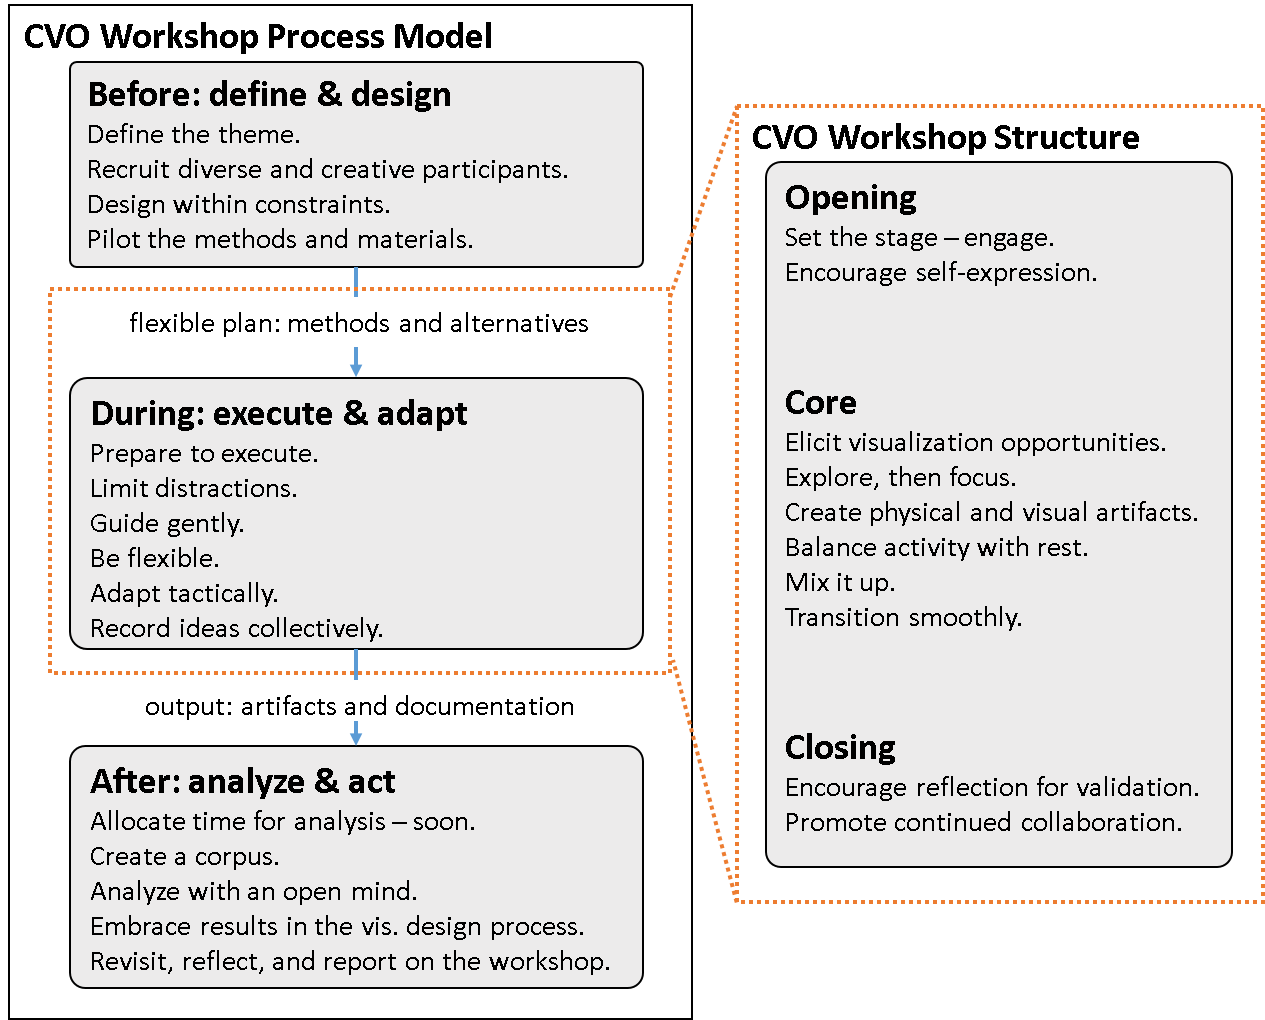
\includegraphics[width=\columnwidth]{figures/final.png}
\caption{The framework's two models are 1) a process model (left) that describes the common actions before, during, and after workshops; and 2) a structure that describes principles for methods used in the beginning, in the middle, and at the end of workshops. In these models, we propose \numberOfGuidelines guidelines for future workshops, summarized here.}
\label{fig:framework-overview}
\end{figure}

The framework proposes two models for describing how to use \workshops: a process model and a workshop structure. The models were adapted from the extensive literature that describes how to use workshops outside of visualization~\cite{CreativeEducationFoundation2015,Brooks-Harris1999,DeBono1983,Dove2016,Gray2010,Hamilton2016,Osborn1953}. 

The process model shown in Fig.~\ref{fig:framework-overview} (left) consists of three stages that describe the actions of using \workshops:
\begin{enumerate}[noitemsep,nolistsep]
    \item {\bf Before: define \& design.} Define the workshop theme and design workshop methods, creating a flexible workshop plan.
    \item {\bf During: execute \& adapt.} Perform the workshop plan, adapting it to participants' reactions in light of the \tactics, generating workshop output as a set of artifacts and documentation.
    \item {\bf After: analyze \& act.} Make sense of the workshop output and use it in the downstream design process.
\end{enumerate}

Nested within the process is the \workshop structure --- Fig.~\ref{fig:framework-overview} (right) --- that identifies key aspects of the methods used in the beginning, middle, and end of workshops:
\begin{enumerate}[nolistsep,noitemsep]
    \item {\bf Opening.} Establish shared context and \interest while promoting \trust, \agency, and \collegiality.
    \item {\bf Core.} Promote creative thinking about the \topic, potentially varying \challenge to maintain \interest.
    \item {\bf Closing.} Provide time for reflection on the \topic and promote continued \collegiality in the collaboration.
\end{enumerate}

The process model and structure are closely connected as shown by the orange box in Fig.~\ref{fig:framework-overview}. As part of the workshop process, we design and execute a workshop plan. This plan follows the workshop structure because it organizes methods into the opening, core, and closing. In other words, the process is about how we use a workshop; the structure is about how methods are organized within a workshop. 

We use the process model and structure to organize the following four sections of this paper. In these sections, we use paragraph-level headings to summarize \numberOfGuidelines actionable workshop guidelines. Additionally, in Supplemental Materials we include a complementary set of \numberOfPitfalls pitfalls that are positioned against these guidelines and the \tactics to further enhance the actionability of the framework.

\section{Before the Workshop: Define \& Design}
\label{sec:before}

Creating an effective \workshop is a design problem: there is no single correct workshop, the ideal workshop depends on its intended outcomes, and the space of possible workshops is practically infinite. Accordingly, workshop design is an iterative process of defining a goal, testing solutions, evaluating their effectiveness, and improving ideas. The framework we have developed here is part of this process. In this section, we introduce four guidelines --- summarized in paragraph-level headings --- for workshop design.

\paragraph{Define the theme.} Just as design starts with defining a problem, creating a \workshop starts with defining its purpose, typically by articulating a concise theme.
An effective theme piques \interest in the workshop through a clear indication of the \topic. It encourages a \mindset of mutual learning among stakeholders. It also focuses on opportunities that exhibit the appropriate {\it task clarity} and {\it information location} of the design study methodology~\cite{Sedlmair2012}. Examples from our work emphasize visualization opportunities (e.g., {\it ``enhancing legends with visualizations''} [\ref{pro:edina}]), domain challenges (e.g., {\it ``identify analysis and visualization opportunities for improved profiling of constraint programs''} [\ref{pro:cp}]), or broader areas of mutual interest (e.g., {\it``explore opportunities for a funded collaboration with phylogenetic analysts"}~[\ref{pro:arbor}]).

Although we can improve the theme as our understanding of the domain evolves, posing a theme early can ground the design process and identify promising participants.

\paragraph{Recruit diverse and creative participants.} \label{par:participants} We recruit participants who have relevant knowledge and diverse perspectives about the \topic. We also consider their openness to \challenge and potential \collegiality.

Examples of effective participants include a mix of frontline analysts, management, and support staff [\ref{pro:graffinity}]; practitioners, teachers, and students [\ref{pro:cp}]; or junior and senior analysts [\ref{pro:lineage}]. We recommend that participants attend the workshop in person because remote participation proved distracting in one workshop~[\ref{pro:arbor}]. Recruiting {\it fellow-tool builders}~\cite{Sedlmair2012} as participants should be approached with caution because their perspectives may distract from the \topic~--- this happened in our workshop that did not result in active collaboration [\ref{pro:updb}].

\paragraph{Design within constraints.} Identifying constraints can help winnow the possibilities for the workshop. Based on our experience, the following questions are particularly useful for workshop design:

\begin{itemize}[nolistsep,noitemsep]

\item Who will use the workshop results? Identifying the primary researcher early in the process is important because he or she will be responsible for the workshop and ultimately use its results. In a workshop where we did not clearly identify the primary researcher, the results went unused [\ref{pro:updb}].

\item How many participants will be in the workshop? We typically recruit 5 to 15 participants --- a majority domain collaborators, but sometimes designers and researchers [\ref{pro:edina},~\ref{pro:htva},~\ref{pro:lineage}~--~\ref{pro:arbor}].

\item Who will help to facilitate the workshop? We have facilitated our workshops as the primary researcher, with the assistance of supporting researchers or professional workshop facilitators. Domain collaborators can also be effective facilitators, especially if the domain vocabulary is complex and time is limited [\ref{pro:cp},~\ref{pro:arbor}].

\item How long will the workshop be? Although we have run workshops that range from half a day [\ref{pro:lineage},~\ref{pro:updb}] to two days [\ref{pro:arbor}], these extremes either feel rushed or require significant commitment from collaborators. We recommend that an effective workshop lasts about one working day.

\item Where will the workshop be run? Three factors are particularly important for determining the workshop venue: a mutually convenient location, a high quality projector for visualization examples, and ample space to complete the methods. We have had success with workshops at offsite locations [\ref{pro:eon},~\ref{pro:htva}], our workplaces, and our collaborators' workplaces [\ref{pro:graffinity}~--~\ref{pro:lineage}].

\item What are additional workshop constraints? Examples include the inability of collaborators to share sensitive data [\ref{pro:htva},~\ref{pro:lineage}] and the available funding.

\end{itemize} 

\paragraph{Pilot the methods and materials.} Piloting methods can ensure that the workshop will generate ideas relevant to the \topic while maintaining appropriate levels of \interest and \challenge. We have piloted methods to evaluate how understandable they are [\ref{pro:eon},~\ref{pro:graffinity}], to test whether they create results that can be used to advance visualization design methodologies [\ref{pro:lineage},~\ref{pro:arbor}], to find mistakes in method prompts [\ref{pro:eon},~\ref{pro:graffinity},~\ref{pro:lineage},~\ref{pro:arbor}], and to ensure that the materials are effective --- e.g., \stickyNotes are the correct size and visualizations are readable on the projector.

It is also useful to pilot workshops with proxy participants, such as researchers~[\ref{pro:graffinity}] or collaborators~[\ref{pro:arbor}]. Feedback from collaborators during pilots has helped us revise the theme, identify promising participants, and refine the workshop methods.

\section{Workshop Structure and Methods}
\label{sec:design}

This section describes guidelines for the methods used in the three phases of the \workshop structure (described in Sec.~\ref{sec:process-and-structure}) --- the opening, core, and closing. It concludes with a summary of an example workshop and resources for additional workshop methods.

\subsection{Workshop Opening}

The workshop opening communicates the goals and guidelines for participants, but it can be more than that. It can foster \agency by encouraging self-expression and idea generation. It can encourage \collegiality and \trust by promoting open communication, acknowledging expertise, and establishing a safe co-owned environment. It can also garner \interest by showing that the workshop will be useful and enjoyable. Two guidelines contribute to an effective opening.

\paragraph{Set the stage --- engage.} \workshops typically open with a short introduction that reiterates the theme and establishes shared context for participants and facilitators. We have introduced workshops as \emph{``guided activities that are meant to help us understand: what would you like to do with visualization?''}~[\ref{pro:graffinity}]. We have also used graphics that summarize the goals of our project, potentially priming participants to engage with the \topic of visualization [\ref{pro:htva}].

The opening can establish principles for creativity~\cite{CreativeEducationFoundation2015,Osborn1953}, potentially fostering \trust and \collegiality. We used the following principles in one of our workshops [\ref{pro:eon}]: 1) all ideas are valid, express and record them; 2) let everyone have their say; 3) be supportive of others; 4) instead of criticizing, create additional ideas; 5) think `possibility' -- not implementation; 6) speak in headlines and follow with detail; and 7) switch off all electronic devices.

Introduction presentations should be kept short to maintain \interest. Passive methods, such as lectures and presentations, can discourage participation at the outset. For example, we started one workshop [\ref{pro:arbor}] with a presentation on the current state of analysis tools. This presentation encouraged participants to passively listen rather than actively explore, establishing a passive mindset that we had to overcome in subsequent methods. An effective opening engages participants.

\paragraph{Encourage self-expression.} We use methods that encourage self-expression to support interpersonal leveling and to act on the creativity principles --- {\it all ideas are valid} and {\it be supportive of others}. Such interpersonal methods help to establish an atmosphere of \trust and \collegiality among participants and facilitators. They can also provide participants with a sense of \agency~\cite{Brooks-Harris1999}.

We have used interpersonal methods that ask participants to sketch ideas while suspending judgment~\cite{Rogers2017} or to introduce themselves through analogies as a potential primer for creativity (see analogy introduction in Sec.~\ref{sec:workshop-methods}). Overall, we use interpersonal methods in the opening to engage participants and facilitators, preparing them for the workshop core.

\subsection{Workshop Core}

In the workshop core, we harness the active and engaged mindset of participants by encouraging them to explore a wide ideaspace before selecting the more promising ideas. The methods in the core potentially generate hundreds of sticky notes, sketches, and other artifacts. Analysis of our experience and relevant literature leads us to suggest five guidelines for an effective core.

\paragraph{Elicit visualization opportunities.} We select workshop methods relevant to the \topic, asking participants about their current analysis challenges, limitations of existing tools, characteristics of their data, or the ways in which they would like to use visualization. This can be achieved by adding a visualization twist to existing design and workshop methods. 

In one workshop [\ref{pro:htva}], for example, we used a method that {\it ``developed user stories, considered relevant datasets, discussed alternative scenarios and sketched solutions"} with our domain collaborators. In retrospect, this method connected the \topic into a more general workshop method, user stories~\cite{Kumar2012}.

% More formally, we refer to the set of all ideas being considered in the workshop as the ideaspace~\cite{Biskjaer2017}, and we select or tailor methods that focus on the ideaspace on the \topic --- exploring possibilities for visualization in a domain.

% \paragraph{Elicit relevant ideas.} We refer to the set of all ideas being considered in the workshop as the ideaspace~\cite{Biskjaer2017}. We select methods that focus the ideaspace on the \topic --- exploring the possibilities for visualization in a specific domain.

% In line with existing visualization practices~\cite{Sedlmair2012}, we use methods that ask participants about their problems, not their envisioned solutions. Example prompts of effective methods include {\it ``What would you like to see in your data?''}~[\ref{pro:eon}], and {\it ``What do you want to do with visualization software?''}~[\ref{pro:cp}]. Responses to these prompts help us discover interesting visualization opportunities.

%This requires judgment to balance focus with flexibility. Allowing for freewheeling discussion and ideation can waste time ~\cite{Chamorro-Premuzic2015}, distract from the \topic, and potentially limit \interest. We have seen this in workshops where participants reported that unconstrained discussions were less effective because they allowed for distractions [\ref{pro:arbor}]. Accordingly, we use methods that have been tailored with domain-specific prompts to produce relevant output. As facilitators, this can feel paradoxical. On the one hand, we use workshops to consider a wide range of possibilities and promote serendipitous discovery. But, exploring a wide range of ideas is made possible through methods remain narrowly focused on the \topic. 

%\paragraph{Look for opportunities.} Remember: we use workshops to discover opportunities for visualization research. To this end, we select methods that focus participant energy on communicating their domain challenges, instead of trying to create visualization solutions. We seldom task workshop participants with designing visualizations. We also balance the use of methods that ask directly about visualizations with more open ended questions. For example, we may select methods that ask, {\it ``What would you like to see in your data?''} or {\it ``What are the exceptional characteristics associated with an excellent visualization solution?''} instead of {\it ``What do you want to do with visualization software?''} The differences are subtle, but, in our experience, the former questions elicit what participants need --- the true opportunities for visualization --- instead of what they want.

\paragraph{Explore, then focus.} We organize the core to first generate ideas using divergent methods that expand the ideaspace. Then, we evaluate ideas using convergent methods that winnow the ideaspace~\cite{Osborn1953}. Using divergent methods early in the core allows us to consider many possibilities while also promoting \agency and maintaining \interest. Then, convergent methods can narrow the ideaspace to the more promising ideas. 

Classifying methods as either divergent or convergent risks oversimplification as individual methods often include both divergent and convergent aspects. Consider our use of brainstorming~\cite{Osborn1953} during one workshop~[\ref{pro:edina}]: we asked participants to record \emph{``problems and successes associated with the current clients on \stickyNotes''} (divergent) and then to share the more interesting ideas (convergent). We classify this method as divergent because it creates ideas, despite the convergent discussion. In contrast, a convergent method may only involve grouping \stickyNotes from previous methods. Overall, in line with existing workshop guidance~\cite{CreativeEducationFoundation2015,DeBono1983,Hamilton2016,Osborn1953}, we judge methods by their intended impact on the ideaspace and organize the core with phases of divergent and convergent methods.

\paragraph{Create physical and visual artifacts.} We select methods by how they encourage participants to write, draw, or otherwise externalize their ideas. Externalizing ideas creates artifacts for us to analyze after the workshop. It aids creative thinking because expressing an idea forces the creator to elaborate it~\cite{Sawyer2006}, and promotes idea sharing that encourages \collegiality.

We consider the artifact materials to be important. Sticky notes are particularly useful because they enable participants to group or rank ideas and potentially to discover emergent concepts in the ideaspace~\cite{Dove2016}. We have used \stickyNotes in almost all of our workshops, often using their color to encode information about which method generated an idea, and their positions to relate, differentiate, or rank ideas. This can help establish consensus. It can also aid post-workshop analysis by recording how ideas evolved and were valued throughout the workshop. Additional materials effective for externalizing ideas include handouts with structured prompts, butcher paper, and poster boards. Using whiteboards is tempting, but ideas are easily lost if the boards are erased.

%It also emphasizes the visualization \mindset by using visual \methods.
We also consider the form of ideas to be important. Effective methods create artifacts relevant to the theme and \topic of visualization. This can be achieved through the use of visual language (see wishful thinking in Sec.~\ref{sec:workshop-methods}) and by encouraging participants to sketch or draw, such as in storyboarding [\ref{pro:eon},~\ref{pro:graffinity},~\ref{pro:cp}]. We see many opportunities to create visual artifacts using existing methods, such as sketching with data~\cite{Walny2015}, constructive visualizations~\cite{Huron2014}, or parallel prototyping~\cite{Roberts2016} approaches.

\paragraph{Balance activity with rest.} Because continuously generating or discussing ideas can be tiring for participants, we structure workshop methods to provide a balance between activity and rest. Specifically, we incorporate passive methods that provide time for incubation, the conscious and unconscious combination of ideas~\cite{Sawyer2006}. 

Passive methods can include short breaks with food and coffee, informal discussions over meals, or methods where participants listen to presentations. When using methods that present ideas, asking participants to record their thoughts and reactions can promote \interest and maintain a feeling of \agency. We have typically used passive methods in full-day workshops [\ref{pro:eon},~\ref{pro:graffinity},~\ref{pro:cp},~\ref{pro:arbor}], but we rely on breaks between methods for shorter workshops [\ref{pro:lineage}].

\paragraph{Mix it up.} We consider the relationships among methods to be important as we strive to balance exploration with focus and activity with rest, while also using many materials for externalizing ideas. Considering methods that vary these factors can provide different levels of \challenge because, for example, methods that require drawing ideas may be more difficult than discussing ideas. Using a variety of methods may also maintain \interest because participants may become bored if too much time is spent on a specific idea.

\paragraph{Transition smoothly.} We avoid potentially jarring transitions between methods to preserve participant \interest. Convergent discussions can be used to conclude individual methods by highlighting the interesting, exciting, or influential ideas. These discussions can promote \collegiality by encouraging communication of ideas, \agency by validating participants' contributions, and \interest in the ideas generated. Convergent discussions also highlight potentially important ideas for researchers to focus on after the workshop.

Convergent methods can also conclude the workshop core by grouping or ranking key ideas. We have used storyboarding to encourage the synthesis of ideas into a single narrative [\ref{pro:eon},~\ref{pro:graffinity},~\ref{pro:cp}]. We have also asked participants to rank ideas, providing cues for analyzing the workshop results [\ref{pro:htva}]. Convergent methods provide a sense of validation, potentially helping to build \trust among researchers and collaborators as we transition to the closing. %In our two-day workshop [\ref{pro:arbor}], we concluded the first day by clustering ideas to identify springboards~\cite{Gordon1961} that we explored in the second day. 

\subsection{Workshop Closing}

The workshop closing sets the tone for continued collaboration. It is an opportunity to promote \collegiality by reflecting on the shared creative experience. It allows for analysis that can potentially identify the more interesting visualization opportunities. The following two guidelines apply to effective closings. % by validating the time and energy that participants have contributed, and by identifying the next steps of action.

\paragraph{Encourage reflection for validation.} We use discussions at the end of workshops to encourage reflection, potentially providing validation to participants and generating information valuable for workshop analysis. We encourage participants to reflect on how their ideas have evolved by asking, \emph{``What do you know now that you did not know this morning?''} [\ref{pro:cp}] or \emph{``What will you do differently tomorrow, given what you have learned today?''} [\ref{pro:eon}]. Responses to these questions can provide validation for the time committed to the workshop. One participant, for example, reported, \emph{``I was surprised by how much overlap there was with the challenges I face in my own work and those faced by others''} [\ref{pro:cp}]. 

%Also, because reflective questions are used to start a discussion, they require participants to rank their thoughts and to talk about the more interesting ones. Recording these ideas can provide important clues for the analysis of workshop artifacts, such as in our neuroscience workshop's closing where discussions about \emph{``multi-hop path queries''} resulted in focusing on connectivity analysis [\ref{pro:graffinity}].

\paragraph{Promote continued collaboration.} We conclude the workshop by identifying the next steps of action --- continuing the \methodology of the collaboration. We can explain how the ideas will be used to move the collaboration forward, often with design methods as we describe in Sec.~\ref{sec:after}. 

We can also ask participants for feedback about the workshop to learn more about their perceptions of visualization and to evaluate the effectiveness of workshop methods --- encouraging the visualization mindset. E-mailing online surveys immediately after a workshop is effective for gathering feedback [\ref{pro:graffinity},~\ref{pro:arbor}].

\begin{figure}
    \centering
    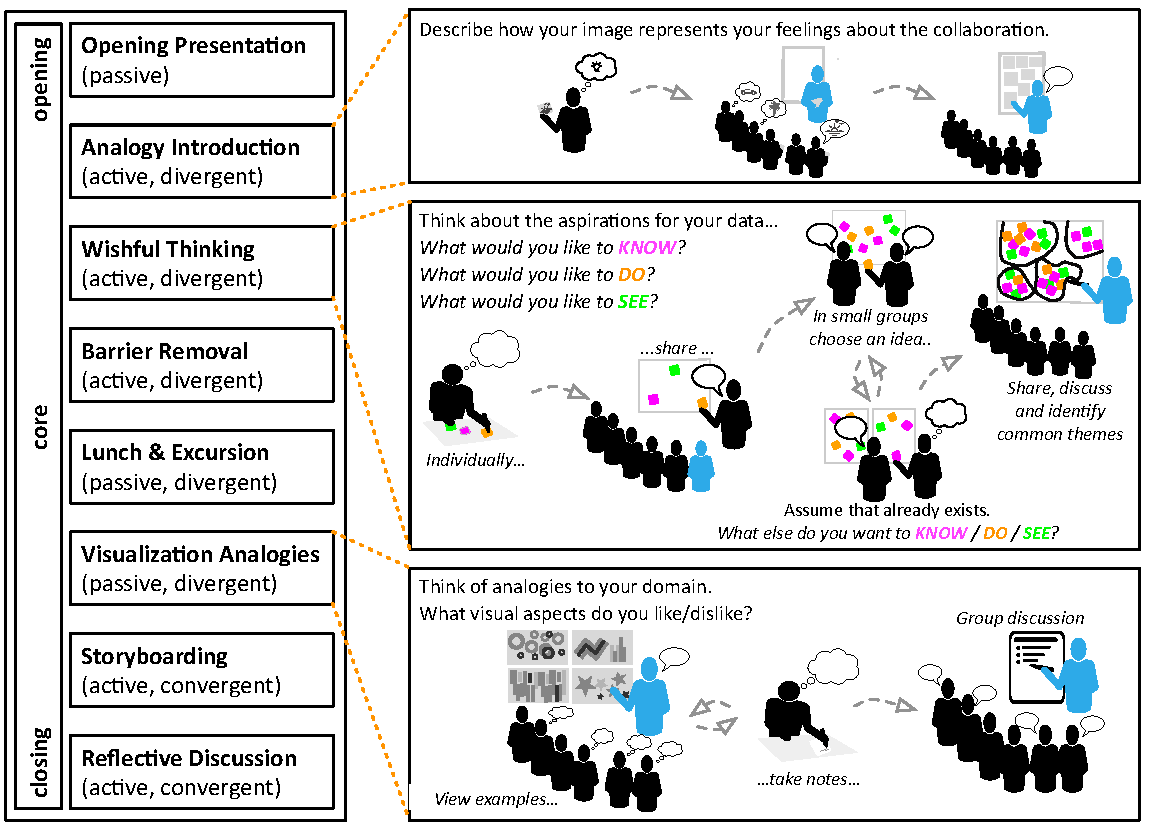
\includegraphics[width=\columnwidth]{figures/workshop.pdf}
    \caption{The eight methods of the full-day, example \workshop (left) with the process of three methods summarized graphically (right). The workshop methods diverge to explore a broad ideaspace before they converge to the more promising ideas. Three of the methods are described in the text and the remainder are explained in the Supplemental Material. The methods can be summarized as: 1) the opening presentation establishes creativity principles; 2) an analogy introduction promotes interpersonal leveling; 3) wishful thinking elicits opportunities for visualization; 4) barrier removal explores those opportunities further; 5) lunch \& excursion provides time for rest and incubation; 6) visualization analogies allows specification of requirements by example; 7) storyboarding summarizes key ideas in a graphic form; and 8) the reflective discussion highlights potentially interesting ideas for workshop analysis. This workshop plan is a starting point for future workshops.}
    \label{fig:example-workshop}
\end{figure}

\subsection{Example Workshop \& Methods}
\label{sec:workshop-methods}
To illustrate the workshop structure, we include an example workshop, shown in Fig.~\ref{fig:example-workshop}. We selected this example because it has proven effective in three of our projects [\ref{pro:eon},~\ref{pro:graffinity},~\ref{pro:cp}]. Here, we describe three methods of this workshop that we have also used successfully in additional workshops [\ref{pro:lineage},~\ref{pro:arbor}], and we refer to the Supplemental Material for descriptions of the remaining five methods. We emphasize that this is a starting place for thinking about workshops, and encourage that methods be adopted and adapted for local context.

To explain the workshop methods, we refer to their process --- the steps of execution~\cite{Biskjaer2017}. This process description abstracts and simplifies the methods because during their execution we adapt the process based on participant reactions and our own judgment of the \tactics. 

\subsubsection*{Analogy Introduction} 

We have used this active, interpersonal, and potentially divergent method in the workshop opening. A process of this method, shown in Fig.~\ref{fig:example-workshop} (right, top), starts with a facilitator posing the analogy introduction prompt, e.g., \emph{``If you were to describe yourself as an animal, what would you be and why?''} [\ref{pro:eon}]. The facilitators and participants then respond to the prompt in turn --- expressing themselves creatively. 

Because everyone responds to the eccentric prompt, this method supports interpersonal leveling that helps to develop \trust and \collegiality among stakeholders. Using analogy can prime participants to think creatively~\cite{Gordon1961}.

This method is simple to execute, and participants report that it has a profound impact on the workshop because of the leveling that occurs. The method helps to establish \trust and that all ideas should be accepted and explored [\ref{pro:graffinity}].

A more topical alternative requires more preparation. We have asked participants to come to the workshop with an image that represents their feelings about the project. Participants have created realistic images, clip-art, and sketches to present and discuss [\ref{pro:htva}]. A visual analogy introduction can help establish the \topic of visualization early in the workshop.

\subsubsection*{Wishful Thinking} 

We have used this divergent, active method early in the workshop core. It is based on creativity methods to generate aspirations~\cite{Hicks2004}. We tailored these methods to visualization by prompting participants with a domain scenario and asking questions: {\it ``What would you like to know? What would you like to do? What would you like to see?''}

One process of this method is shown in Fig.~\ref{fig:example-workshop} (right, middle). First, we introduce the prompt and participants answer the know/do/see questions individually on \stickyNotes. Next, participants share ideas in a large group to encourage \collegiality and cross-pollination of ideas. Then, participants form small groups and try to build on their responses by selecting interesting ideas, assuming that they have been completed, and responding to the know/do/see questions again --- increasing the \challenge. Finally, we lead a convergent discussion to highlight interesting ideas and to transition to the next method.

We encourage participants to record answers to the know/do/see questions on different color \stickyNotes because each prompt provides information that is useful at different points in the design process. Participants describe envisaged insights they would like \emph{to know} and analysis tasks that they would like \emph{to do}. Asking what participants would like {\it to see} is often more of a \challenge, but ensures that a \topic of visualization is established early.

We tailor the prompt to the workshop theme and project goals. For example, we asked energy analysts about long term goals for their project --- \emph{``aspirations for the Smart Home programme\ldots''} They generated forward-thinking ideas, e.g., to better understand the value of the data [\ref{pro:eon}]. In contrast, we asked neuroscientists about their current analysis needs --- \emph{``suppose you are analyzing a connectome\ldots''} They created shorter term ideas, e.g., to see neuron connectivity [\ref{pro:graffinity}].

%The ideas generated in this method can cascade through the workshop. They can be ranked by importance or grouped to find emergent themes. They can also be elaborated in subsequent methods, such as Barrier Removal in the example workshop.

\subsubsection*{Visualization Analogies} 

We have used this divergent, initially passive method later in the workshop core because it promotes incubation while allowing participants to specify visualization requirements by example.  Similar to analogy-based creativity methods~\cite{Gordon1961} and the visualization awareness method~\cite{Koh2011}, we present a curated collection of visualizations and ask participants to individually record analogies to their domain and to specify aspects of the visualizations that they like or dislike. We have used this method repeatedly, iteratively improving its process by reflecting on what worked in a number of our workshops [\ref{pro:edina}~--~\ref{pro:cp},~\ref{pro:arbor}]. 

%  %This activity is low on \collegiality and \challenge but is intended to have positive effects on \trust and \interest.

One process of this method is shown in Fig.~\ref{fig:example-workshop} (right, bottom). First, we provide participants with paper handouts that contain a representative image of each visualization --- we have encouraged participants to annotate the handouts, externalizing their ideas [\ref{pro:graffinity},~\ref{pro:cp},~\ref{pro:arbor}]. Next, we present the curated visualizations on a projector and ask participants to think independently about how each visualization could apply to their domain and record their ideas. Then, we discuss these visualizations and analogies in a large group.

We curate the example visualizations to increase \interest and establish participants' \trust in our visualization expertise. We have used visualizations that we created (to show authority and credibility); those that we did not create (for diversity and to show knowledge of the field); older examples (to show depth of knowledge); challenging examples (to stretch thinking); playful examples (to support engagement and creativity); closely related examples (to make analogies less of a \challenge); and unrelated examples (to promote more challenging divergent thinking).

The discussions during this method have expanded the workshop ideaspace in surprising ways, including \emph{``What does it mean for legends to move?''} [\ref{pro:edina}], \emph{``What does it mean for energy to flow?''} [\ref{pro:eon}], and \emph{``What does it mean for neurons to rhyme?''}~[\ref{pro:graffinity}]. Although this method is primarily passive, participants report that it is engaging and inspiring to see the possibilities of visualization and think about how such visualizations apply to their domain.

% Because this method is initially passive, it gives participants room to think individually. They reported that it is engaging and inspiring to see the broad possibilities of visualization and discuss how such visualizations apply to their domain.

\subsubsection*{Additional Methods \& Resources} 

We introduce the example workshop and methods as starting points for future workshops. Yet, the workshop design space is practically infinite and design should be approached with creativity in mind.

To help researchers navigate the design space, our Supplemental Material contains a list of \numberOfExampleMethods example methods that we have used or would consider using in future workshops. For these methods, we describe their process, their influence on the workshop ideaspace, their level of activity, and their potential impact on the \tactics for effective workshops.

We have also found other resources particularly useful while designing workshops. These include books~\cite{CreativeEducationFoundation2015,Gray2010,Hamilton2016,Hohmann2007,Kumar2012,Michalko2006} and research papers~\cite{McFadzean1998,McKenna2014,Sanders2005}. Although these resources target a range of domains outside of visualization, we tailor the workshop methods such that they encourage a visualization mindset and focus on the \topic of visualization opportunities.
\section{During The Workshop: Execute \& Adapt}
\label{sec:during}

Continuing the \workshop process model shown in Fig.~\ref{fig:framework-overview}, we execute the workshop plan. This section proposes five guidelines for workshop execution.

\paragraph{Prepare to execute.} We prepare for the workshop in three ways: resolving details, reviewing how to facilitate effectively, and checking the venue. We encourage researchers to prepare for future workshops in the same ways.

We prepare by resolving many details, such as inviting participants, reserving the venue, ordering snacks for breaks, making arrangements for lunch, etc. Brooks-Harris and Stock-Ward~\cite{Brooks-Harris1999} summarize many practical details that should be considered in preparing for execution. Our additional advice is to promote the visualization mindset in workshop preparation and execution.

We prepare by reviewing principles of effective facilitation, such as acting professionally, demonstrating acceptance, providing encouragement, and using humor~\cite{CreativeEducationFoundation2015,Brooks-Harris1999,Gray2010,Hamilton2016,Stanfield2002}. We also assess our knowledge of the domain because, as facilitators, we will need to lead discussions. Effectively leading discussions can increase \collegiality and \trust between stakeholders as participants can feel that their ideas are valued and understood. In cases where we lacked domain knowledge, we recruited collaborators to serve as facilitators [\ref{pro:cp},~\ref{pro:arbor}]. 

We also prepare by checking the venue for necessary supplies, such as a high quality projector, an Internet connection (if needed), and ample space for group activity. Within the venue, we arrange the furniture to promote a feeling of co-ownership and to encourage \agency~--- a semi-circle seating arrangement works well for this~\cite{Vosko1991}. A mistake in one of our workshops was to have a facilitator using a podium, which implied a hierarchy between facilitators and participants, hindering \collegiality~\cite{Rogers2016}.

\paragraph{Limit distractions.} Workshops provide a time to step away from normal responsibilities and to focus on the \topic. Accordingly, participants and facilitators should be focused on the workshop without distractions, such as leaving for a meeting. 

Communicating with people outside of the workshop --- e.g., through e-mail --- commonly distracts participants and facilitators. It should be discouraged in the workshop opening (e.g., \emph{switch off all electronic devices}). Principles in the workshop opening, however, should be justified to participants. Also, facilitators should lead by example at the risk of eroding \trust and \collegiality.

% \paragraph{Get out of the way.} After the workshop opening establishes a creative atmosphere and fosters engagement, participants commonly take initiative in completing the workshop methods. Hence, we use the word {\it facilitator} to describe the individuals guiding the workshop because their role is to {\it facilitate} the exploration of ideas as opposed to {\it lead} or {\it command} the participants. To an extent, facilitating a workshop is like conducting an interview because we should stay quiet and try to keep the participants talking or generating ideas. 

\paragraph{Guide gently.} While starting execution, the workshop opening can establish an atmosphere in which participants take initiative in completing methods. It is, however, sometimes necessary to redirect the participants in order to stay focused on the \topic. Conversations that deviate from the workshop theme should be redirected. In one workshop [\ref{pro:graffinity}], participants were allowed to discuss ideas more freely, and they reported in feedback that, {\it ``We had a tendency to get distracted [during discussions].''} In a later workshop [\ref{pro:arbor}], we more confidently guided discussions, and participants reported  \emph{\it ``We were guided and kept from going too far off track \ldots this was very effective.''}

However, guiding participants requires judgment to determine whether a conversation is likely to be fruitful. It also requires us to be sensitive to the \tactics~--- e.g., how would redirecting this conversation influence \collegiality or \agency? Redirection can be jolting and can contradict some of the guidelines (e.g., \emph{all ideas are valid}). We can prepare participants for redirection with another guideline during the workshop opening: \emph{Facilitators may keep you on track gently, so please be sensitive to their guidance.} 

\paragraph{Be flexible.} As we guide participants to stay on topic, it is important to be flexible in facilitation. For example, we may spend more time than initially planned on fruitful methods or cut short methods that bore participants. 

Following this guideline can also blur the distinction between participants and facilitators. In one workshop [\ref{pro:htva}], participants proposed a method that was more useful than what was planned. Thus, they became facilitators for this part of the workshop, which reinforced \agency and maintained the \interest of all stakeholders in the project. In the future, we may explore ways to plan this type of interaction, perhaps encouraging participants to create their own methods. 

\paragraph{Adapt tactically.} As we guide the workshop, we interpret group dynamics and adapt methods to the changing situation. We can be forced to adapt for many reasons, such as a failing method (\emph{nobody feels like an animal this morning}; \emph{sticky notes don't stick}), a loss of \interest (\emph{there is no energy}; \emph{the room is too hot}; \emph{we had a tough away day yesterday}); a lack of \agency (\emph{some participants dominate some tasks}); or an equipment failure ({\it projector does not work}; {\it no WiFi connection to present online demos}~[\ref{pro:eon}]). Designing the workshop with alternative methods in mind --- perhaps with varying degrees of \challenge~--- can ensure that workshop time is used effectively.

\paragraph{Record ideas collectively.} Remember: conversations are ephemeral and anything not written down will likely be forgotten. We therefore encourage facilitators and participants to document ideas with context for later analysis. Selecting methods to create physical artifacts can help with recording ideas. As described in Sec.~\ref{sec:design}, externalizing ideas on \stickyNotes and structured prompts has been effective in our workshops and addresses the visualization mindset. 

We are uncertain about the use of audio recording to capture workshop ideas. Although it can be useful for shorter workshops [\ref{pro:lineage}], it can require tremendous time to transcribe before analysis~\cite{Lloyd2011}. Also, recording audio effectively can be challenging as participants move around during the workshop.

It can be useful to ensure that facilitators know that they are expected to help document ideas. A pilot workshop can help with this. In at least one of our projects [\ref{pro:cp}], a pilot workshop may have reduced the note taking pressure on the primary researcher by setting clear expectations that all facilitators should help take notes.


% \paragraph{Assemble alternatives.}If participants do not find a method helpful, they may propose their own as when analysts proposed walking through visualization analysis scenarios in place of a planned method [\ref{pro:htva}]. Facilitators should be prepared for flexibility, perhaps by having alternative methods planned or by being ready to improvise. It requires judgment to deviate from the plan, and the design considerations should be considered on-the-fly as the workshop adapts to participant responses.


\section{After the Workshop: Analyze \& Act}
\label{sec:after}

After the \workshop, we analyze its output and use the results of that analysis to influence the on-going collaboration. Here, we describe five guidelines for this analysis and action. 

\paragraph{Allocate time for analysis --- soon.} Effective \workshops generate rich and inspiring artifacts that can include hundreds of \stickyNotes, posters, sketches, and other documents. The exact output depends on the methods used in the workshop. Piloting methods can help prepare researchers for the analysis. Regardless, making sense of this output is labor intensive, often requiring more time than the workshop itself. Thus, it is important that we allocate time for analysis, particularly within a day of the workshop, so that we can analyze the workshop output while the experiences are still fresh in our memory.

\paragraph{Create a corpus.} We usually start analysis by creating a digital corpus of the \workshop output. We type or photograph the artifacts, organizing ideas into digital documents or spreadsheets. Through this process, we become familiar with key ideas contained in the artifacts. The corpus also preserves and organizes the artifacts, potentially allowing us to enlist diverse stakeholders --- such as facilitators and collaborators --- in analysis [\ref{pro:graffinity}]. This can help in clarifying ambiguous ideas or adding context to seemingly incomplete ideas.

\paragraph{Analyze with an open mind.} Because the ideas in the workshop output will vary among projects, there are many ways to analyze this corpus of artifacts. We have used qualitative analysis methods --- open coding, mindmapping, and other less formal processes --- to group artifacts into common themes or tasks [\ref{pro:eon},~\ref{pro:graffinity}~--~\ref{pro:updb}]. Quantitative analysis methods should be approached with caution as the frequency of an idea provides little information about its potential importance.

We have ranked the themes and tasks that we discovered in analysis according to various criteria, including novelty, ease of development, potential impact on the domain, and relevance to the project [\ref{pro:eon},~\ref{pro:graffinity}--~\ref{pro:lineage}]. In other cases~[\ref{pro:edina},~\ref{pro:htva}], workshop methods generated specific requirements, tasks, or scenarios that could be edited for clarity and directly integrated into the design process. 

We encourage that analysis be approached with an open mind because of the many ways to make sense of the workshop data, including some approaches that we may not yet have considered.

\paragraph{Embrace results in the visualization design process.} Similarly, \workshop results can be integrated into visualization methodologies and processes in many ways. We have, for example, run additional workshops that explored the possibilities for visualization designs [\ref{pro:edina},~\ref{pro:eon}]. We have applied traditional user-centered design methods, such as interviews and contextual inquiry, to better understand collaborators' tasks that emerged from the workshop~[\ref{pro:graffinity}]. We have created prototypes of varying fidelity, from sketches to functioning software [\ref{pro:graffinity}~--~\ref{pro:lineage}], and we have identified key aims in proposals for funded collaboration~[\ref{pro:arbor}]. 

In all of these cases, our actions were based on the reasons why we ran the workshops, and the workshop results profoundly influenced the direction of our collaboration. For example, in our collaboration with neuroscientists~[\ref{pro:graffinity}], the workshop helped us focus on graph connectivity, a topic that we were able to explore with technology probes and prototypes of increasing fidelity, ultimately resulting in new visualization tools and techniques.

\paragraph{Revisit, reflect, and report on the workshop.} The \workshop output is a trove of information that can be revisited throughout (and even beyond) the project. It can be used to document how ideas evolve throughout applied collaborations. It can also be used to evaluate and validate design decisions by demonstrating that any resulting software fulfills analysis needs that were identified in the workshop data~[\ref{pro:edina}~--~\ref{pro:lineage}]. Revisiting workshop output repeatedly throughout a project can continually inspire new ideas.

In our experience creating this paper, revisiting output from our own workshops allowed us to analyze how and why to use \workshops.  We encourage researchers to reflect and report on their experiences using \workshops, the ways in which workshops influence collaborations, and ideas for future workshops. We hope that this framework provides a starting point for research into these topics.
\section{Discussion}
\label{sec:discussion}

This section discusses implications and limitations of \workshops and the research methodology of critically reflective practice.

\subsection{Limitations of CVO Workshops}

Our experience across diverse domains --- from cartography to neuroscience --- provides evidence that \workshops are a valuable and general method for fostering the visualization mindset while creating artifacts that advance visualization methodologies. We argue that they achieve these goals through the use of \methods that appropriately emphasize the \topic of visualization opportunities while accounting for (inter)personal factors, including \agency, \collegiality, \challenge, \interest, and \trust. 

Yet, workshops may not be appropriate in some scenarios. Because using workshops requires researchers to ask interesting questions and potentially lead discussions about their collaborators' domain, we caution the use of workshops as the first method in a project. Traditional user-centered approaches should be used to learn domain vocabulary and explore the feasibility of collaboration. In the project that did not result in ongoing collaboration~[\ref{pro:updb}], we lacked the domain knowledge needed to effectively design the workshop. Also, our collaborators were too busy to meet with us before the workshop, which should have been a warning about the nature of the project. Accordingly, we recommend researchers evaluate the preconditions of design studies~\cite{Sedlmair2012} in projects where they are considering workshops.

We also recognize that workshops may not be well received by all of the stakeholders. In a full-day workshop [\ref{pro:graffinity}], one participant reported that {\it ``Overall, it was good, but a bit long and slightly repetitive.''} Similarly, after another full-day workshop [\ref{pro:cp}], one participant said {\it ``There was too much time spent expanding and not enough focus \ldots discussions were too shallow and nonspecific.''} Nevertheless, both workshops were generally well received by stakeholders as they allowed us to explore a broad space of visualization opportunities. We can, however, improve future workshops by ensuring that the methods are closely related to the \topic and that we facilitate workshops in a way that provides appropriate \agency to all of the stakeholders.

More generally, whether workshops can enhance creativity is an open question~\cite{Nickerson1999,Sawyer2006}. 
Creativity is a complex phenomenon studied from many perspectives, including design~\cite{Shneiderman2005}, psychology~\cite{Sawyer2006}, sociology~\cite{Lubart1999}, and biology~\cite{Martindale1999}. The results of several controlled experiments indicate that group-based methods can reduce creativity~\cite{Bouchard1969,Mullen1991}. Yet, critics of these studies argue that they rely on contrived metrics and lack ecological validity~\cite{Hewett2005,Mayer1999}. Experimentally testing the relationship between workshops and creativity is beyond the scope of this paper. Instead, we focus on understanding and communicating how we use \workshops in applied collaborations.


\subsection{Critically Reflective Practice}

Throughout this project, we wrestled with a fundamental question: how can we rigorously learn from our diverse, collective experience? We first examined measurable attributes of workshops, such as their length, number of participants, and quantity of ideas generated. However, our workshops were conducted over 10 years in applied settings with no experimental controls. More importantly, it is difficult, if not impossible, to measure how ideas influence collaborations. Quantitative analysis, we decided, would not produce useful knowledge about how to use \workshops. 

We also considered qualitative research methodologies and methods, such as grounded theory~\cite{Corbin1990} and thematic analysis~\cite{Braun2006}. These approaches focus on extracting meaning from externalized data, but the the most meaningful and useful information about workshops resided in our collective, experiential knowledge. We therefore abandoned analysis methods that ignore (or seek to suppress) the role of experience in knowledge generation. 

We found critically reflective practice to be an appropriate approach, providing a methodology to learn from the analysis of experience, documentation, and existing theory, while allowing for the use of additional analysis methods~\cite{Brookfield1998,Thompson2008}. Due to the nature of reflection, however, the framework is not exhaustive, predictive, or objective. Nevertheless, it is consistent with our experience, grounded in existing theory, and, we argue, useful for future visualization research.

Yet, the use of reflective practice may raise questions about the validity of this work. After all, can the framework be validated without experimental data? We emphasize our choice of the term {\it framework}~\cite{Jabareen2008} because we intend for it to be evaluated by whether it provides an interpretive understanding of \workshops. Our position is that it achieves this goal because it enabled us to learn from our experience using workshops on 3 continents over the past 10 years. For example, we used the framework to identify and organize \numberOfPitfalls pitfalls to avoid in future workshops --- they are described in the Supplemental Material. This framework, however, is only a snapshot of our current understanding of \workshops, which will continue to evolve with additional research, practice, and reflection.

Given that this work results from the subjective analysis of our experience, we recognize that there could also be questions about its trustworthiness. Therefore, to increase the trustworthiness of our results, we provide an audit trail~\cite{Carcary2009,Lincoln1985} of our work that contains a timeline of our analysis and our experience as well as diverse artifacts, including comparative analysis of our workshops, presentations outlining the framework, early written drafts of our framework, and structured written reflection to elicit ideas from all of this paper's coauthors. This audit trail, in Supplemental Material, summarizes and includes \numberOfAudits of the reflective artifacts, culled from the original set to protect the privacy of internal discussions and confidential materials from our domain collaborators. 

In future reflective projects, we plan to establish guidelines that encourage transparency of reflective artifacts through  mechanisms to flag documents as on- or off-the-record. Because our research and meta-analysis would have been impossible without well-preserved documentation, we hope that the audit trail inspires future thinking on how to document and preserve the decisions in visualization collaborations. We put forth both the audit trail and our documented use of critically reflective practice as secondary contributions.
\section{Conclusion and Future Work} 
\label{sec:conclusion}

This paper contributes a framework for using workshops in the early stages of applied visualization research. The framework consists of two models for \workshops~--- a process model and a workshop structure. The framework also includes \numberOfGuidelines actionable guidelines for future workshops and a validated example workshop. 

We support the framework with Supplemental Material that includes extended details about the example workshop, \numberOfExampleMethods additional example workshop methods, \numberOfPitfalls pitfalls to avoid in future workshops, and an analysis timeline and audit trail documenting how we developed the framework during a 2-year reflective collaboration. We hope that this framework inspires others to use and report on \workshops in applied visualization research.

Further thinking on the framework reveals opportunities for developing \workshop \methods that emphasize the visualization \mindset. For example, inspired by the Dear Data project~\cite{Lupi2016}, we could ask participants to create graphics that reveal something about their daily life in the week before the workshop. The Dear Data Postcard Kit~\cite{Lupi2017} offers guidance and materials for creating data visualizations about personal experiences, which could be adopted in \workshops.

We also hope to better understand the role of data in \workshops. Visualization methodologies stress the importance of using real data early in collaborative projects~\cite{Lloyd2011,Sedlmair2012}. Our workshops, however, have focused participants on their perceptions of data rather than using real data because working with data is time consuming and unpredictable. In some projects, we incorporated data into the design process by using a series of workshops spaced over weeks or months, providing time for developers to design prototypes between workshops [\ref{pro:edina} -- \ref{pro:htva}]. This development between workshops was expensive in terms of time and effort. But time moves on, and we may be able to reliably use data in workshops with new technologies and techniques, e.g., visualization design tools~\cite{Wongsuphasawat2016}, declarative visualization languages~\cite{Satyanarayan2017}, constructive visualization~\cite{Huron2014}, and sketching~\cite{Walny2015}.

Additionally, in this paper we focused on workshops to elicit visualization opportunities in the early stages of applied work. Exploring how the framework could be influenced by and extended for workshops that correspond to other stages of applied work --- including the creation and analysis of prototypes, the exploration of data, or in the deployment, training and use of completed systems --- may open up opportunities for using creativity in visualization design and research.
\acknowledgments{We are grateful to the participants, facilitators, and fellow researchers in all of our workshops. We thank the following people for their feedback and contributions to this work: the anonymous reviewers, Graham Dove, Tim Dwyer, Peter Hoghton, Christine Pickett, David Rogers, Francesca Samsel, members of the Vis Design Lab at the University of Utah, and members of the giCentre at City, University of London. This work was supported in part by NSF Grant IIS-1350896. }

% \acknowledgments{We thank everyone who has been involved in our workshops as participants or facilitators. We also thank Graham Dove, Tim Dwyer, Carolina Nobre, Alexander Lex, Peter Hoghton, Curtis Lisle, Francesca Samsel, David Rogers, Nina McCurdy, Robert Marc, Jimmy Moore, and the members of the Vis Design Lab at the University of Utah for their feedback and support.}

\bibliographystyle{abbrv}
%%use following if all content of bibtex file should be shown
%\nocite{*}
\bibliography{test,workshops}

\end{document}
